\documentclass[12pt]{article}
\usepackage[utf8]{inputenc}
\usepackage{gensymb}
\usepackage{textcomp}
\usepackage{mathtools}
\usepackage{amssymb}
\usepackage{todonotes}
\title{Machine Learning Engineer Nanodegree Capstone Project}
\author{Mateusz Bednarski}
\date{\today}


\usepackage{graphicx}
\graphicspath{ {images/} }

\DeclareMathOperator*{\argmax}{arg\,max}
\usepackage{hyperref}


\begin{document}

\maketitle



\section{Introduction}

Domain for my capstone project is solving classical control problems. I have selected two: Cart pole and Mountain car. Both of them are well-know problems in computer science study. For purposes of this project I decided to make use of OpenAI Gym (LINK). Gym is set of environments simulating various tasks. It provides ready to use simulators and frameworks for comparing algorithms. Also it does have environments with Cart Pole\footnote{\url{https://gym.openai.com/envs/CartPole-v1}} and Mountain Car\footnote{\url{https://gym.openai.com/envs/MountainCar-v0}} which are well-know reinforcement-learning problems. There is a few reasons I have chosen this setup:

\begin{itemize}
\item For first, reinforcement learning interested me the most, so I want to get deeper into this.

\item Both selected problems are well-know and used to compare algorithms perfomance
\item OpenAI provides leaderborads for each environement, making result comparison easy
\item 
OpenAI provides problem implementations, thus I can focus only on RL part.
\item Both problems have continous state space, so basic tabular Q-learing will not work. I need to examine more sophisticated techniques
\item I want to solve two problems instead of one, in order to see how solution will generalize (not being strongly problem-specified)
\end{itemize}


Let's briefly describe both selected problems.

\section{Problem Statement}
\subsection{Cart Pole}

There is a frictionless track, and a vehicle attached to it. Vehicle can move left or right. On top of it, pole is attached. Cart cannot stay at place. Goal is to keep pole vertical and not allow it to fall or run out of track by moving cart left/right. Environment already provides reward (only one): +1 every step that pole is upright

Simulation ends either when pole is deviated over $15\degree$ from vertical or cart is 2.4 units away from the center of the track.

Environment is solved when pole is keeped for 200 time steps.

\begin{figure}[h]
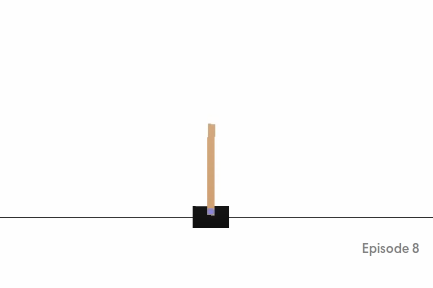
\includegraphics[width=0.5\textwidth]{cartpole_intro.png} 
\centering
\caption{The Cart Pole environment from OpenAI.}
\end{figure}


\subsection{Mountain Car}
There is a track between two mountains. Vehicle starts in a valley between them. The goal is to climb right top. Car does not have enough power to do this just riding right - it needs to build momentum. 

The only reward of -1 is given every timestep. There is no reward on approach top. But this is sufficent to minimize time spent, as simulation ends when reached right mountain.

\begin{figure}[h]
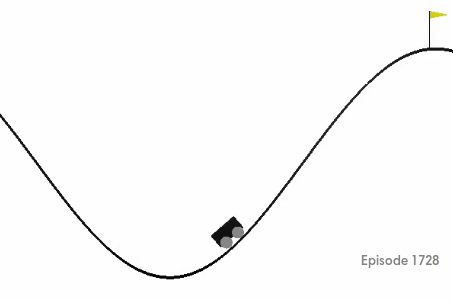
\includegraphics[width=\textwidth]{mountaincar_intro.png} 
\centering
\caption{The Mountain Car environment form OpenAI.}
\end{figure}


\subsection{Evaluation metric}

For measuring performance I will use moving average of cumulative reward for last 100 episodes.

\section{Changes against proposal}
TBD

\section{Analysis}
\subsection{Data Exploration}

As it is a reinforcement learning problem, there is no dataset understood in classical way. Instead, I explored mechanics of problems more deeply. For each problem, data about states distribution for was generated using random action selection. There is a need to be careful with this data - for random walking probably, many states will not be visited much often. However it provides an overview.

\subsubsection{Cart Pole}

Action space is a discrete, finite set $A = \{0,1\}$ where 0 means go left, and 1 go right.
Space state is a vector of four real values. 
\begin{multline}
 S = (s_0, s_1, s_2, s_3) \in \mathbb{R}^4 \\
-4.8 < s_0 < 4.8 \\
-\infty < s_1 < \infty \\
-0.42 < s_2 < 0.42 \\
-\infty < s_3 < \infty \\
\end{multline}

Meaning is following: $s_0$ - cart position, $s_1$ cart velocity, $s_2$ - pole angle and $s_4$ - pola angular velocity.


\subsubsection{Mountain Car}
Action space is a discrite, finite set $A = \{0,1,2\}$ wchich means consecutively move accelerate left, do nothing, accelerate right. Space state is a 2-dimensional vector.

\begin{multline*}
 S = (s_0, s_1) \in \mathbb{R}^2 \\
-1.2 < s_0 < 0.6 \\
-0.07 < s_1 < 0.07
\end{multline*}

$s_0$ is position and $s_1$ is velocity.

\subsubsection{Visualization}

\begin{figure}[h]
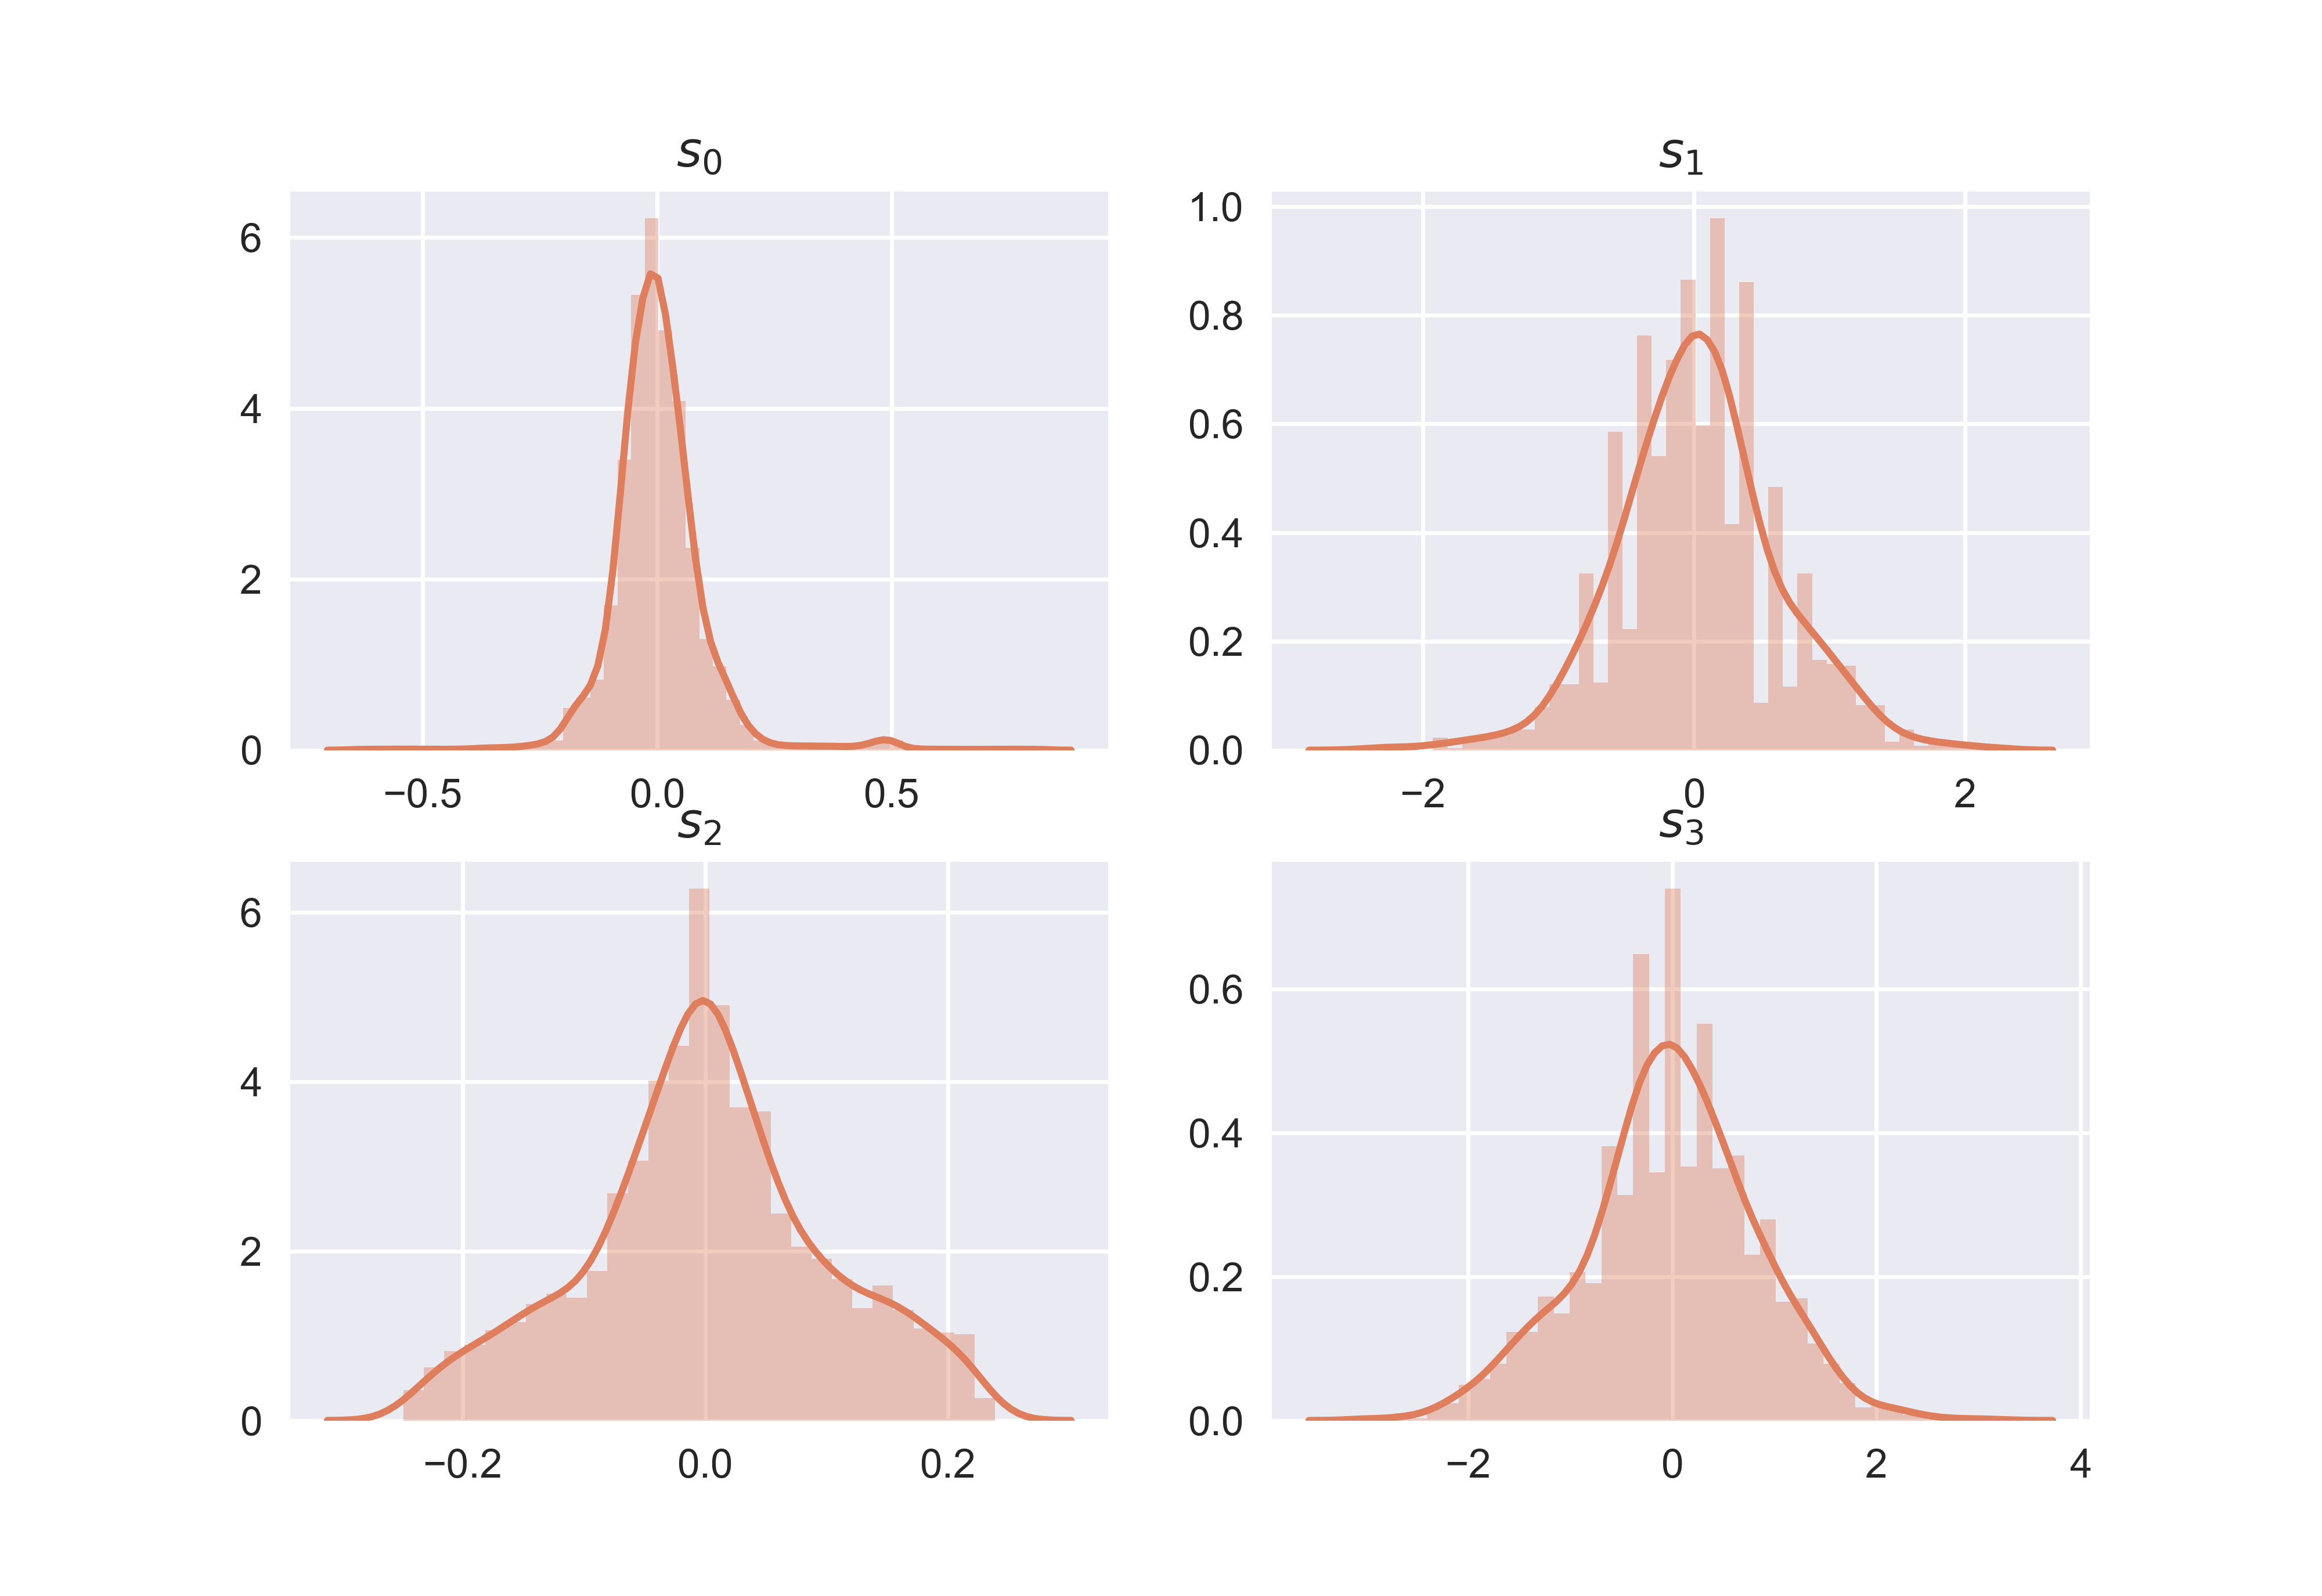
\includegraphics[width=\textwidth]{exploratory_cartpole.png} 
\centering
\caption{Cart Pole distribution of $S$ for random agent is somewhere around normal. Simulation runned for 100 episodes.}
\end{figure}

\begin{figure}[h]
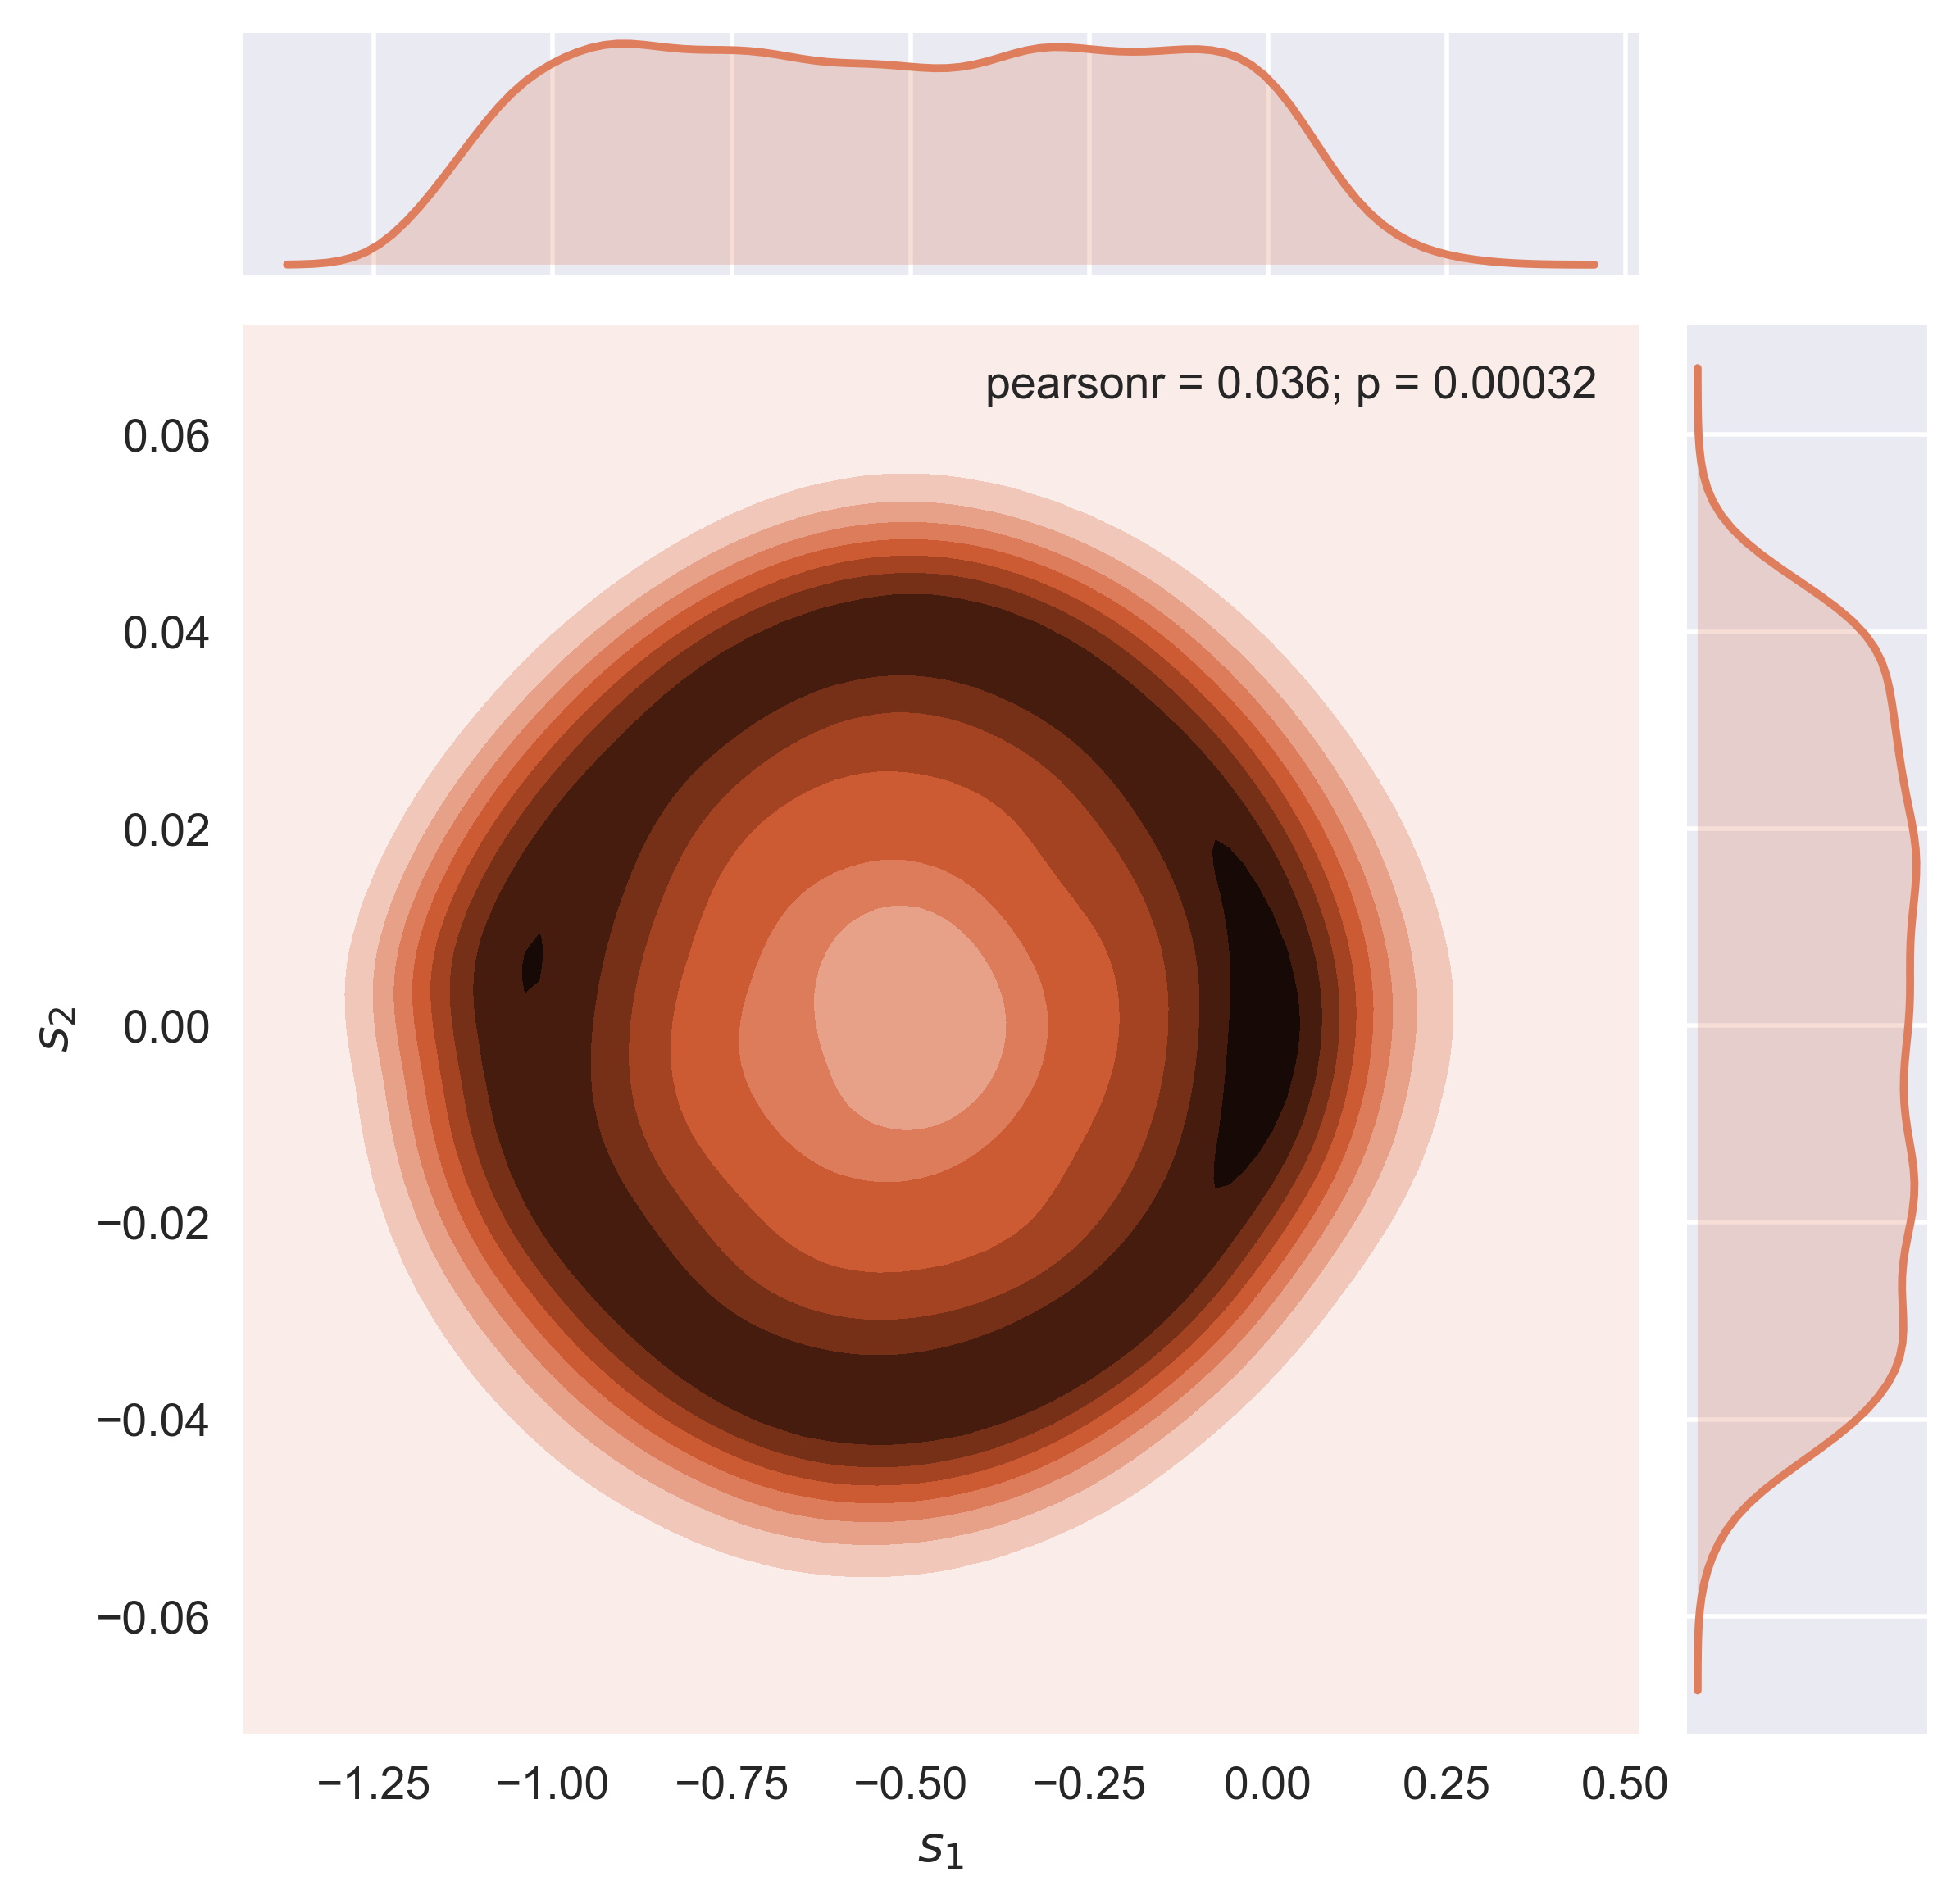
\includegraphics[width=\textwidth]{exploratory_mountaincar.png} 
\centering
\caption{Mountain Car distribution of $S$ for random agent. Simulation runned for 10000 steps.}
\end{figure}

\subsection{Space size}

Before, I said that space consists of real numbers. Given that, space state size (for both problems) would be uncountably infinite. However, during to machine representation of real numbers it is not exactly true. In typical implementation, \emph{float} can handle one of $2^{52}$ values \footnote{\url{http://stackoverflow.com/a/8875223}}. Storing Q-table for 2 actions and one real-valued state would take:



\begin{equation}
|Q| = |S \times A| = |S| \times |A| = 2^{52} \cdot 2 = 2^{53} = 9007199254740992
\end{equation}

Which requires 36 PB of memory. Only for that simple problem. It definetely makes this unsolvable by tabular Q-learning.

\subsection{Algorithms}

Because Q-space ($S \times A$) is infinite in size, it is impossible to use Q lookup table. There are at least two approaches to deal wit this problem. First, is to replace Q table with a function $h(s,a) \rightarrow \mathbb{R}$, that will approximate $Q(s, a)$ values. Therefore, the goal is to find a function $h(s, a)$, that will return a Q-value for a given pair $(s,a)$. The second one, is to discretize continuous space. Both of them were implemented.
\\[12pt]
This approach allows to:
\begin{enumerate}
\item Handle continuous Q-space
\item Generalize knowledge to unvisited states
\item Provides robustness – similar Q-states will have similar Q-values
\end{enumerate}

\subsection{Linear model}
The most basic model will be to use linear function:

\begin{equation}
h(s, a) = \sum_i^n f_i(s, a)w_i
\end{equation}

There is a need to describe $f_i$. As we can see, $h(s,a)$ is a linear combination of $n$ $f_i$ functions. Each $f_i$ function can represent a different feature. Feature in the most simple cases, can be just observations. For example, if Q-space is defined as 

\begin{equation}
\begin{aligned}
&S = \mathbb{R}^4 \\
&A = \{0, 1\} \\
&Q = S \times A
\end{aligned}
\end{equation}

we could create following $f_i$ functions

\begin{equation}
\begin{aligned}
&f_0(s, a) = 1 \\
&f_1(s, a) = s_1 \\
&f_2(s, a) = s_2 \\
&f_3(s, a) = s_3 \\
&f_4(s, a) = s_4 \\
&f_5(s, a) = a \\
\end{aligned}
\end{equation}


Phase of creating $f_i$ functions is called \emph{feature engineering}. Used features are described in detail in section data preprocessing.

Therefore, update rule will be following:
\begin{equation}
\begin{aligned}
\delta&=(R(s,a,s')+\gamma V(s',a'))-Q(s,a) \\
w_i &\leftarrow w_i+\alpha \delta f_i (s,a)
\end{aligned}
\end{equation}

Where V is defined as:
\begin{equation}
V(s',a' )=\max_{a'}Q(s',a')
\end{equation}

After each step, we are updating weights in function approximating q-values.

Another possibility is to use 2 separate $Q(s,a)$ functions - one per action. In our example that would be separate $Q_a$ for each action:

\begin{equation}
\begin{aligned}
&Q(s, a) = Q_a(s) \\
&Q_1(s) = \sum_i^n f_i(s)w_{1i} \\
&Q_2(s) = \sum_i^n f_i(s)w_{2i} \\
\end{aligned}
\end{equation}

This can be useful because each action have a separate model and they will not interact with each other. I suppose linear model might be not sufficient to handle relations between all possible actions. From the other hand, non-linear model will be more prone to overfitting. However, there is possibility to use engineered features in order to make linear model perform better. This was implemented in project. More details in preprocessing section. 

\subsection{Space discretization using kNN and SARSA}
Another approach is to discretize space state. As we cannot store all continuous values we can discriteze the space. This will reduce size to finite, and allow us to use eg. tabular Q-learning. However, for this problem I used SARSA (Which is on-policy, in contrast of off-policy qlearning - I'll explain difference later) with kNN.

\subsubsection{Discretization}

First step for kNN-SARSA is to normalize input space. I explain this in preprocessing section. At this point, let's assume that state space is normalized into d-dimensional vector of real values in range $(-1, 1)$.

For each dimmension, we place $p$ \emph{nodes}, arranged unformly \footnote{Also other arrange schemes are possible e.g. Gaussian}. Therefore, for $n$ dimensional space, with $p$ nodes and $|A|$ actions we have Q-space with size:

\begin{equation}
|Q| = p^d \cdot |A|
\end{equation}

\subsubsection{Acquiring Q-value for a q-state}

We introduce parameter $k$ just as in normal kNN algorithm witch tells how meany nearest neighbors we consider. For observed state $s$ we find $k$ nearest nodes (using euclidean distance \footnote{Why we normalize}) and for each of them we compute its influence on our observed state. $n$ menas a neighbor node.

\begin{equation}
\forall knn, \quad knn_i = \frac{1}{1+\text{distance}(knn, s)^2}
\end{equation}

Given that, we transform $knn_i$ values in a way to make them sum up to $1$.

\begin{equation}
\forall knn, \quad w_i = \frac{knn_i}{\sum knn_i}
\end{equation}

The $w$ values, becomes weights how much each neighbor node is affecting observed state. Given that q-value for action $a$ in observed state $s$ is:

\begin{equation}
V(a, s) = \sum_{knn} Q(knn, a)w_i
\end{equation}

\subsubsection{Choosing action}

Action to perform is selected by computing $V(a, s)$ for each action $a$ in observed state $s$ and choosing one wiht highest value.

\begin{equation}
\argmax_a V(a, s)
\end{equation}

There is no $\epsilon$ because for exploration-exploitation I use optimistic initial Q-values.

\subsubsection{On-policy learning}

\todoin{Explain the difference}

\subsubsection{Eligibility traces}

\todoin{Describe}

\subsubsection{Learning}

\subsection{Benchmark}

Select result to compare.

\end{document}

